\documentclass[\main.tex]{subfiles}

\chapter{Produto Final}
\begin{singlespace}
\minitoc
\end{singlespace}
\vspace{40pt}

No momento da redação deste documento, o projeto encontra-se no seu estado final. Posto isto, a aplicação
conta com um sistema de gestão de utilizadores e sessões, ou seja, um utilizador, depois de registado, pode
realizar o \textit{login} para que tenha acesso à sua interface de jogo com as suas informações pessoais
(nome, resultado atual e melhor resultado obtido).\par
Na figura 4.1 e 4.2 estão representados o componente de login e registo de um utilizador,
respetivamente.\par

\begin{figure}[h!]
\centering
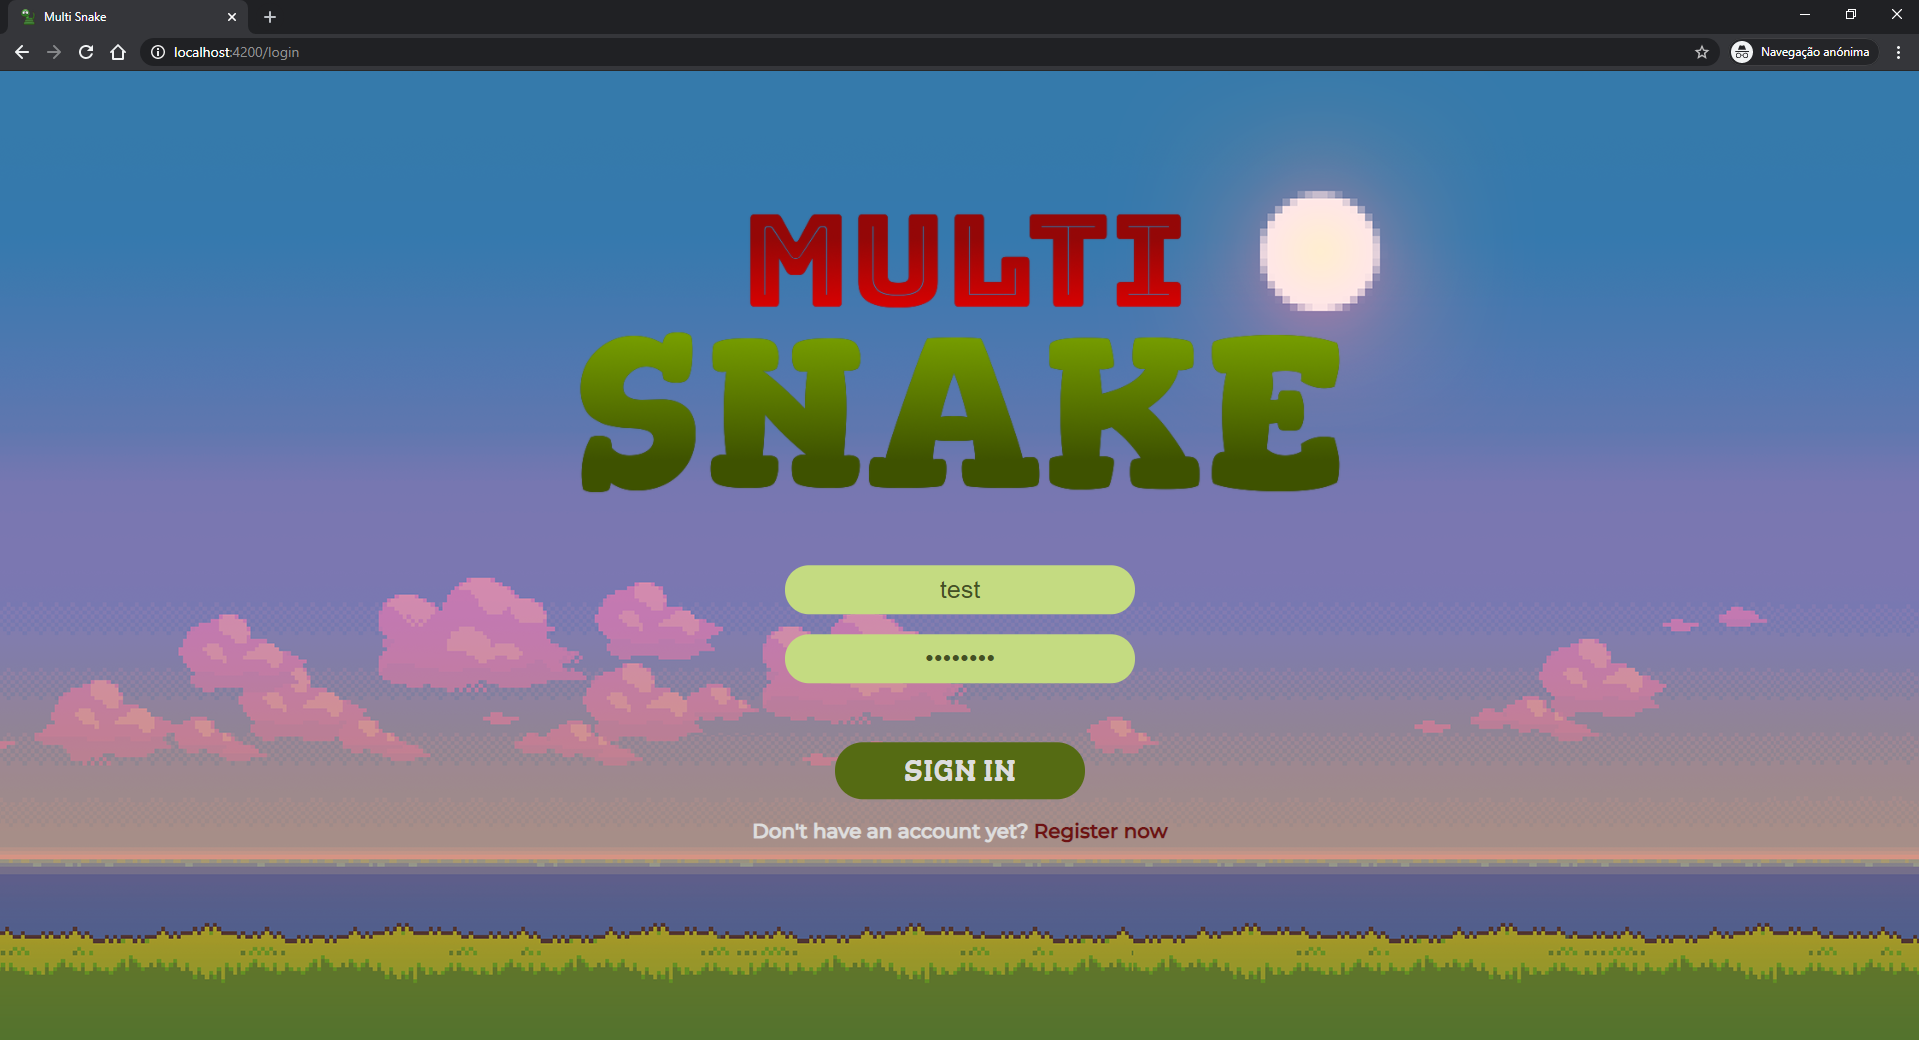
\includegraphics[width=0.9\linewidth]{../private_assets/Login.png}
\caption{Componente de login de utilizadores}
\end{figure}

\newpage

\begin{figure}[h!]
\centering
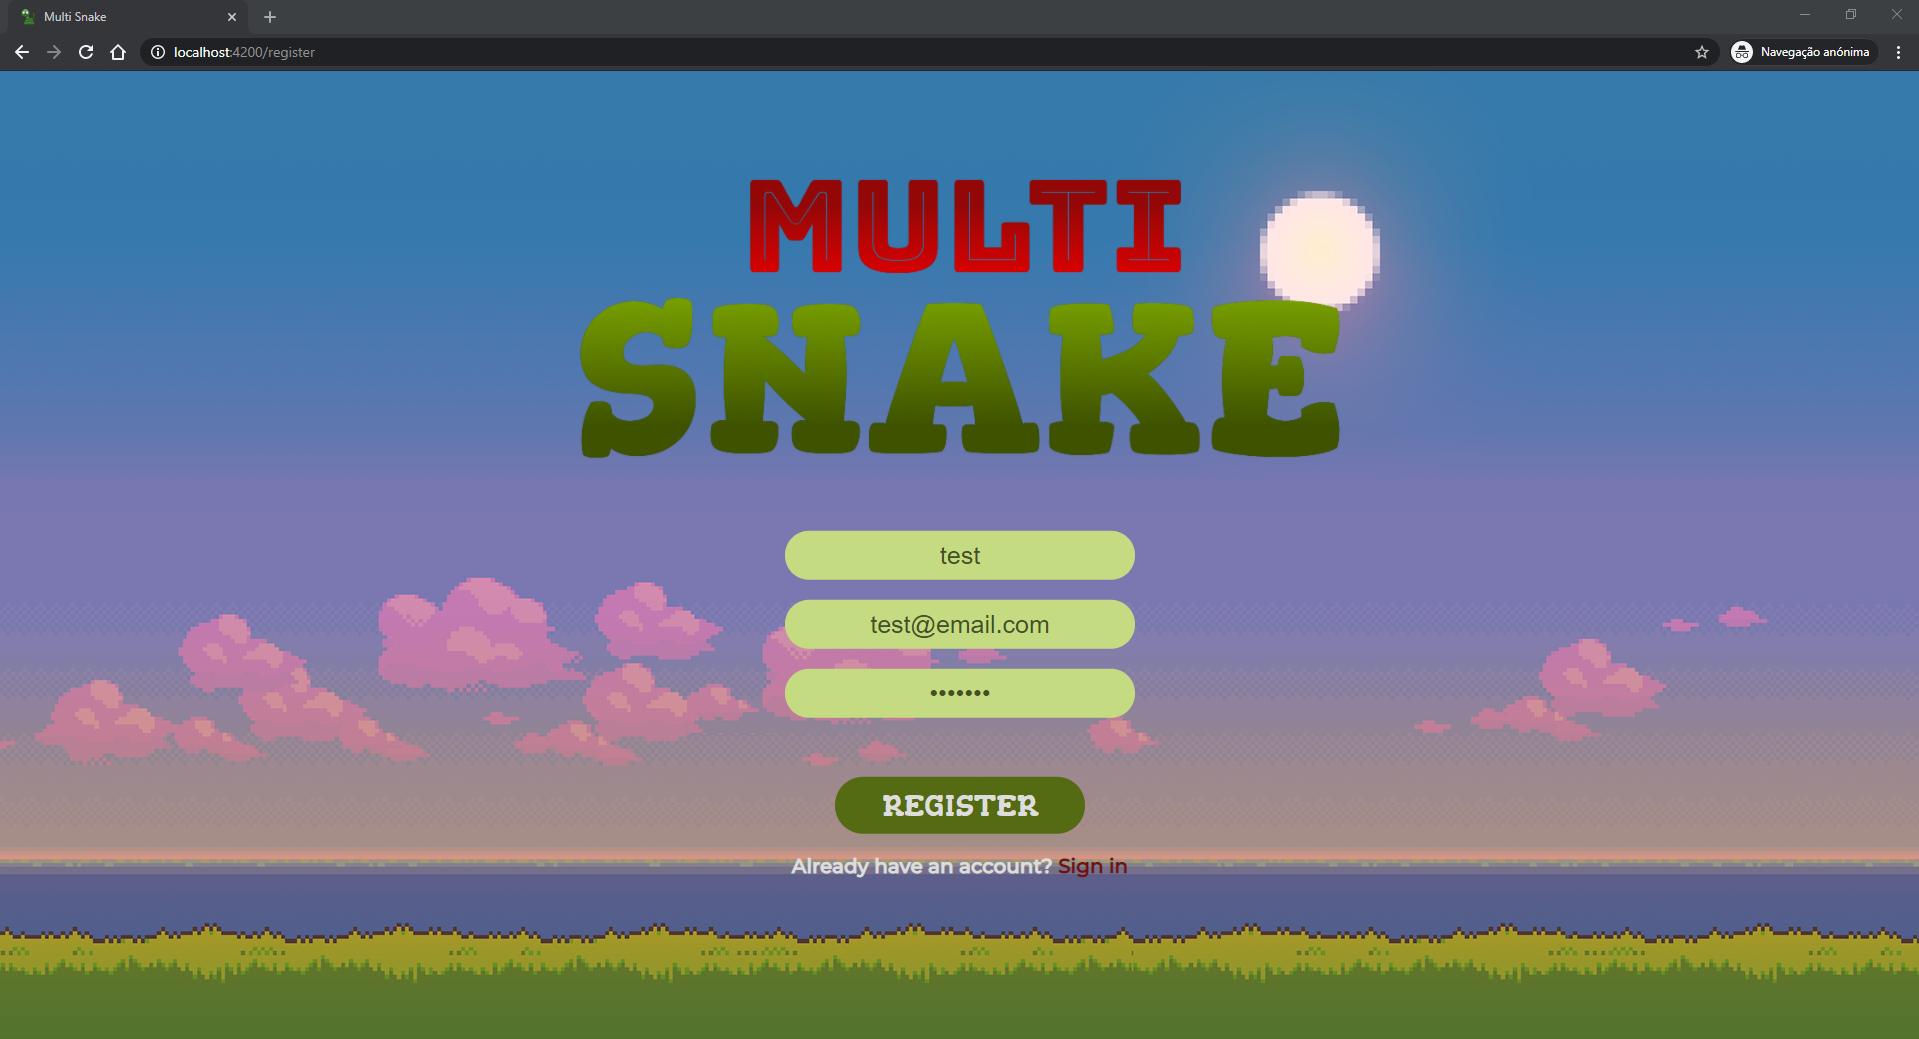
\includegraphics[width=0.9\linewidth]{../private_assets/Register.png}
\caption{Componente de registo de utilizadores}
\end{figure}

Para terminar, qualquer utilizador que se encontre neste ponto da aplicação pode disfrutar do jogo da cobra
multi jogador. A figura 4.3 demonstra a aplicação com apenas um utilizador a jogar e com as suas
informações no cabeçalho da página \par

\begin{figure}[h!]
\centering
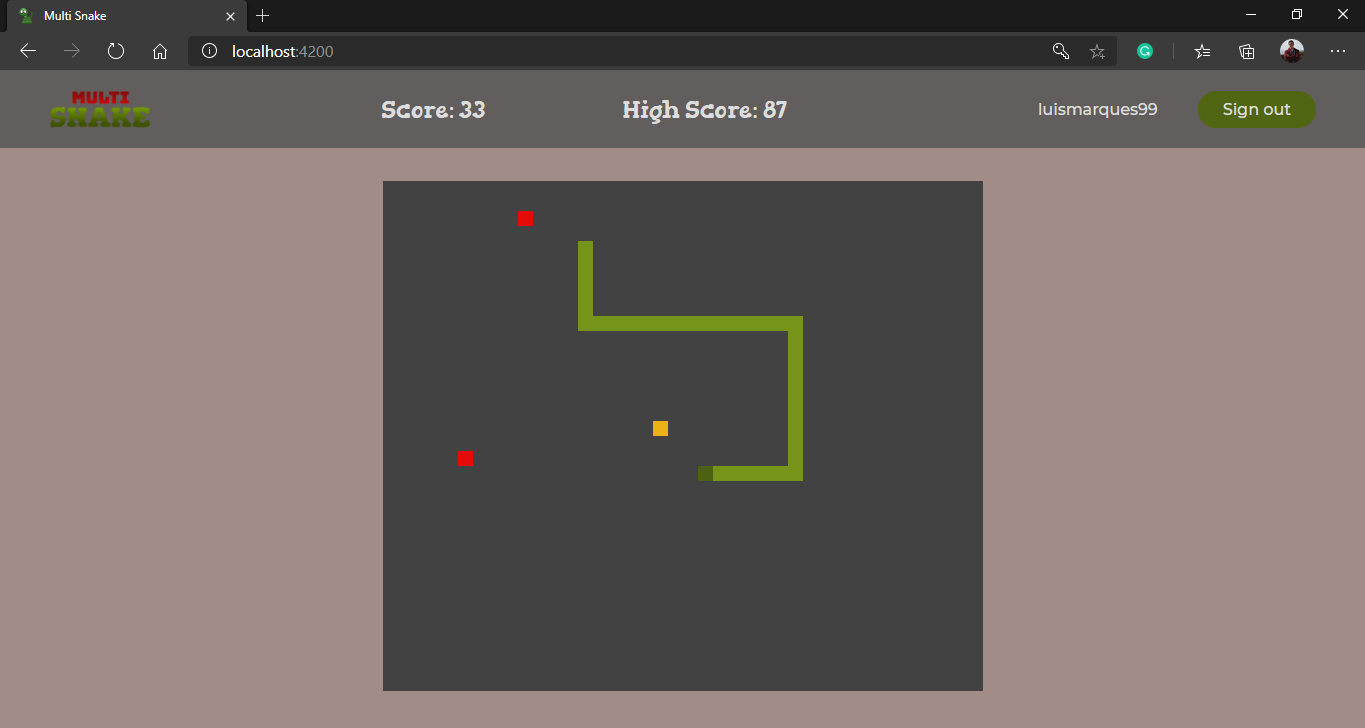
\includegraphics[width=0.9\linewidth]{../private_assets/MultiPlayer1.png}
\caption{Página privada de um utilizador com uma versão multiplayer do jogo da cobra}
\end{figure}

Como pode ser observado na imagem anterior, as maçãs podem assumir duas cores: vermelha, que significa que é
uma maçã comum e apenas dá um ponto à cobra; amarela, que representa uma maçã "dourada" com alguma raridade
em aparecer e resulta em cinco pontos para a cobra.\par

\newpage

Quando mais que um utilizador está a jogar, podem ser vistas duas cores nas cobras. A primeira é verde, que
representa a cobra do utilizador. A segunda é laranja que representa as restantes cobras a competir com os
restantes jogadores.\par
Na figura 4.4 está demonstrada a utilização da aplicação por dois utilizadores diferentes, com sessão
iniciada.\par

\begin{figure}[h!]
\centering
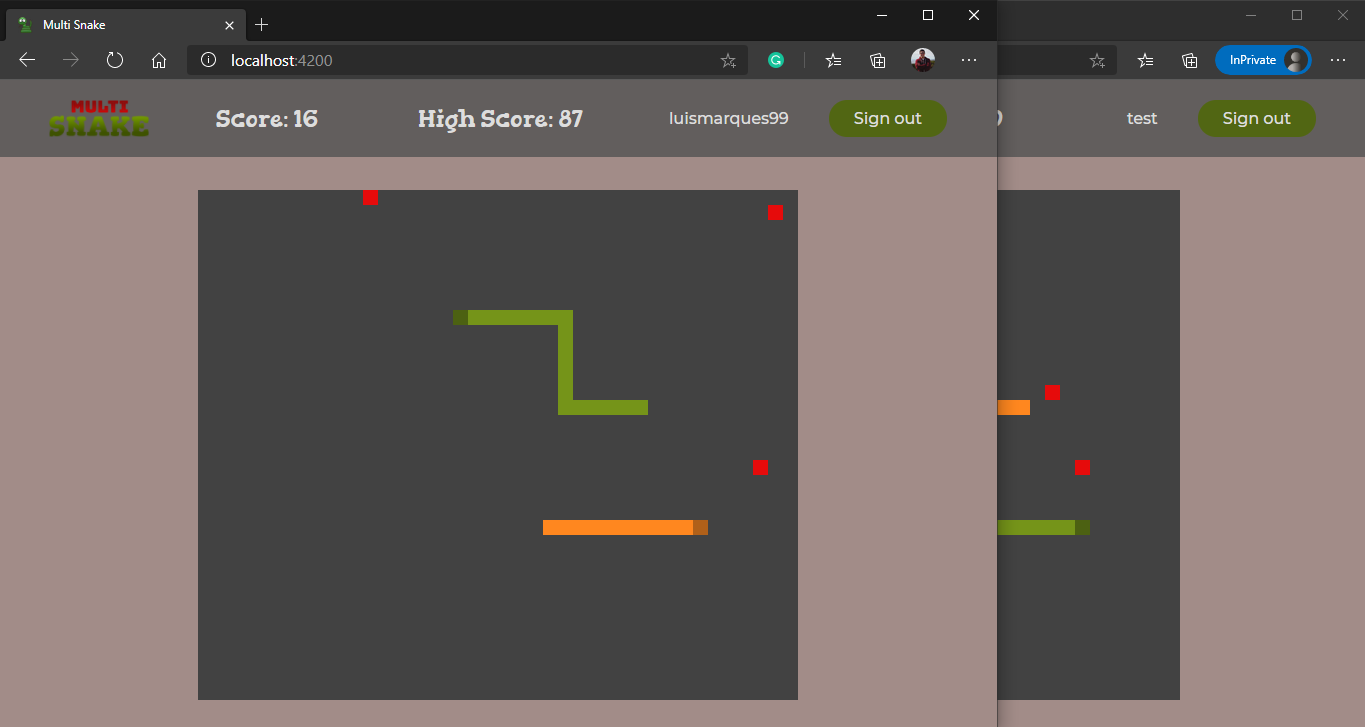
\includegraphics[width=0.9\linewidth]{../private_assets/MultiPlayer2.png}
\caption{Jogo da cobra multiplayer com dois utilizadores diferentes}
\end{figure}

\newpage